\documentclass{article}
\usepackage{amsmath, amssymb, graphicx}
\usepackage[margin=1in]{geometry}
\usepackage{amsmath,amssymb}   % For math symbols
\usepackage{graphicx}          % For including figures
\usepackage{booktabs}          % For nicer tables
\usepackage{hyperref}          % For clickable links (references)
\usepackage{color}             % (Optional) For color if needed
\title{\textbf{Exploring the Google PageRank Algorithm}}
\author{Enrique Rivera, Christine Kim \\ University of Texas at Austin}
\date{\today}


\begin{document}

\maketitle

%------------------------------------------
%  Abstract
%------------------------------------------
\begin{abstract}
In this paper, we investigate the Google PageRank algorithm by studying small examples of directed web graphs. 
We construct the hyperlink matrix \(H\), discuss its properties as a stochastic matrix, implement the iterative PageRank process, 
and illustrate how Theorem 4.9 (the Perron--Frobenius result) ensures convergence to a unique steady-state vector. 
We compare iterative solutions to direct eigenvalue-based solutions and conclude by discussing how one might 
improve a website's ranking and potential future extensions to the algorithm.
\end{abstract}

%------------------------------------------
%  Keywords
%------------------------------------------
\textbf{Keywords:} PageRank, Markov chain, stochastic matrix, eigenvalue, linear algebra

%------------------------------------------
%  Introduction
%------------------------------------------
\section{Introduction}
The PageRank algorithm, developed by Sergey Brin and Larry Page, revolutionized how web pages 
are ranked by their ``importance.'' The core idea is that a page is ``important'' if it is linked to by 
other important pages. Mathematically, one models the web as a directed graph and constructs 
a \emph{hyperlink matrix} \(H\). This matrix then defines a Markov chain whose steady-state 
distribution reflects the ``popularity score'' of each page.

In this report, we follow the exercises in \cite{Sullivan2025Linear} (see Section 4.9.1) to:
\begin{enumerate}
  \item Construct the hyperlink matrix \(H\) for the sample webs in Figures 4.3 and 4.4.
  \item Implement the iterative PageRank update \(x_{k+1} = H x_k\).
  \item Show conditions for \(H\) to be a column-stochastic matrix.
  \item Apply Theorem 4.9, illustrating how the unique steady state can be found by solving the eigenvalue problem \(Hx = x\).
  \item Compare the iterative and direct-eigenvalue approaches to find the steady-state rank vector.
  \item Explore the ``random surfer'' modification and discuss possible improvements to the algorithm.
\end{enumerate}

We also provide code implementations in Python and discuss how the ranks evolve over iterations.

%------------------------------------------
%  Hyperlink Matrix Construction
%------------------------------------------
\section{Hyperlink Matrix Construction (Exercises 4.95--4.97)}

In Figure~4.3, we have a web of six pages. Each page's ``out-links'' determine the columns of the hyperlink matrix 
$H \in \mathbb{R}^{6 \times 6}$. Recall that if page $j$ links to $m$ different pages, each of those $m$ pages 
receives an entry $\tfrac{1}{m}$ in column $j$, while non-linked pages receive $0$ in that column.

\begin{figure}[h]
  \centering
  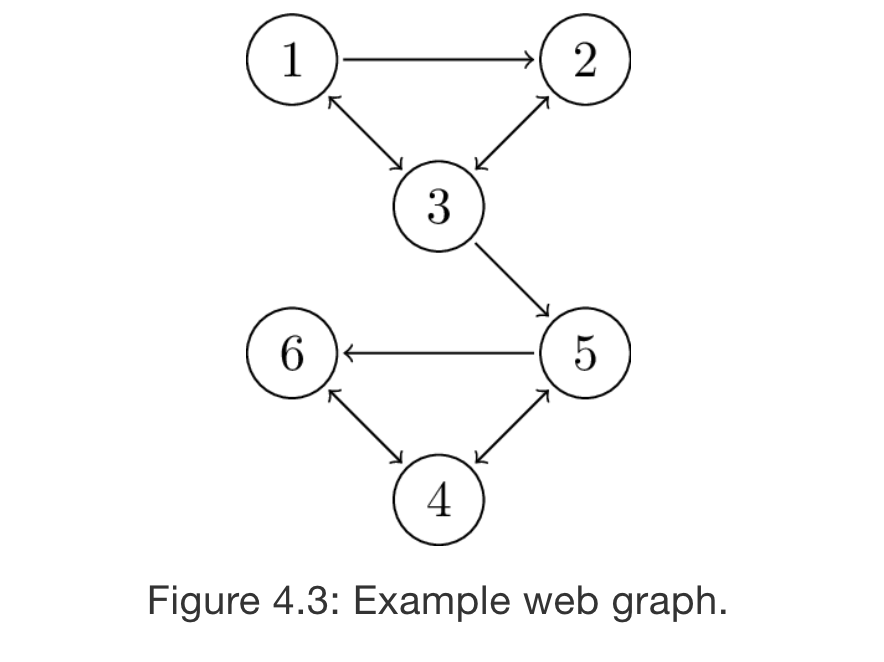
\includegraphics[width=0.65\textwidth]{img/Node_Tree_4.3.png}
  \caption{%
    The first example web shown in Figure~4.3, which consists of six pages labeled 1 through 6.
  }
  \label{fig:Node_Tree_4.3}
\end{figure}

Based on the diagram, the out-links for each page (indexed as 1 through 6) are:
\begin{itemize}
  \item Page 1 links to pages 2 and 3.
  \item Page 2 links to page 3.
  \item Page 3 links to pages 1, 2, and 5.
  \item Page 4 links to pages 5 and 6.
  \item Page 5 links to pages 4 and 6.
  \item Page 6 links to pages 3 and 4.
\end{itemize}
This makes the out-degree of page~1 equal to 2, page~2 equal to 1, and so on.

\bigskip

Hence, the full $6 \times 6$ hyperlink matrix $H$ is:
\[
H 
= 
\begin{pmatrix}
0      & 0      & \tfrac{1}{3} & 0          & 0          & 0 \\
\tfrac{1}{2} & 0      & \tfrac{1}{3} & 0          & 0          & 0 \\
\tfrac{1}{2} & 1      & 0           & 0          & 0          & \tfrac{1}{2} \\
0      & 0      & 0           & 0          & \tfrac{1}{2} & \tfrac{1}{2} \\
0      & 0      & \tfrac{1}{3} & \tfrac{1}{2} & 0          & 0 \\
0      & 0      & 0           & \tfrac{1}{2} & \tfrac{1}{2} & 0
\end{pmatrix}.
\]

\noindent
Each column $j$ sums to 1, as every page $j$ ``distributes'' its total probability mass $\tfrac{1}{\text{outdeg}(j)}$ 
among the pages it links to. Note that entries of $H$ are all nonnegative, so $H$ is a \emph{column-stochastic matrix}.

\paragraph{Why is $H$ Stochastic?}
A matrix is column-stochastic if
\begin{enumerate}
  \item All entries are nonnegative, and 
  \item The entries in each column sum to 1.
\end{enumerate}
Since each page $j$ has outdegree $\text{outdeg}(j)$ and we assign $\tfrac{1}{\text{outdeg}(j)}$ to each linked page, the sum 
in column $j$ is exactly 1. Thus $H$ is indeed a valid hyperlink matrix. This completes Exercises~4.95--4.97.


%------------------------------------------
%  Iterative PageRank & Plot
%------------------------------------------
\section{Iterative Process and Plot (Exercise 4.96)}

We now demonstrate how to implement the PageRank iterative process 
\[
x_{k+1} \;=\; H \, x_{k}
\]
for the matrix \(H\) found in Section~\ref{sec:MatrixConstruction}. 
Since our web contains 6~pages, we set the initial state to
\[
x_0 \;=\; \left(\tfrac{1}{6}, \tfrac{1}{6}, \tfrac{1}{6}, \tfrac{1}{6}, 
\tfrac{1}{6}, \tfrac{1}{6}\right)^T.
\]
We apply the update \(x \leftarrow Hx\) repeatedly and observe convergence 
to a steady-state vector. In practice, we stop either after a fixed number of 
iterations (e.g., 10--15) or once successive iterates differ by less than 
some tolerance (e.g., \(\|x_{k+1} - x_k\|\le 10^{-8}\)).

\subsection{Python Example}
Below is a minimal Python script illustrating the iterative update and a simple 
plot of each page's rank versus iteration number. 
Be sure to replace the \verb|H| array with the final 6$\times$6 matrix 
from Section~\ref{sec:MatrixConstruction}.

\begin{verbatim}
import numpy as np
import matplotlib.pyplot as plt

# Hyperlink matrix (6x6) - fill in your actual entries:
H = np.array([
    [0,   0,   1/3, 0,   0,   0],
    [1/2, 0,   1/3, 0,   0,   0],
    [1/2, 1,   0,   0,   0,   1/2],
    [0,   0,   0,   0,   1/2, 1/2],
    [0,   0,   1/3, 1/2, 0,   0],
    [0,   0,   0,   1/2, 1/2, 0]
], dtype=float)

# Number of pages:
n = 6

# Initial rank vector (uniform):
x0 = np.ones(n) / n

# Number of iterations:
num_iters = 10

# Store each iterate for later plotting:
x_vals = [x0]
x = x0.copy()
for k in range(num_iters):
    x = H @ x
    x_vals.append(x)

x_vals = np.array(x_vals)

# Print the final approximate PageRank:
print("Steady-state (approx.) after", num_iters, "iterations:")
print(x)

# Plot the evolution of each page's rank:
for i in range(n):
    plt.plot(x_vals[:, i], marker='o', label=f"Page {i+1}")

plt.xlabel("Iteration")
plt.ylabel("Rank Value")
plt.title("PageRank Convergence via Iteration")
plt.legend()
plt.show()
\end{verbatim}



\begin{figure}[h]
      \centering
      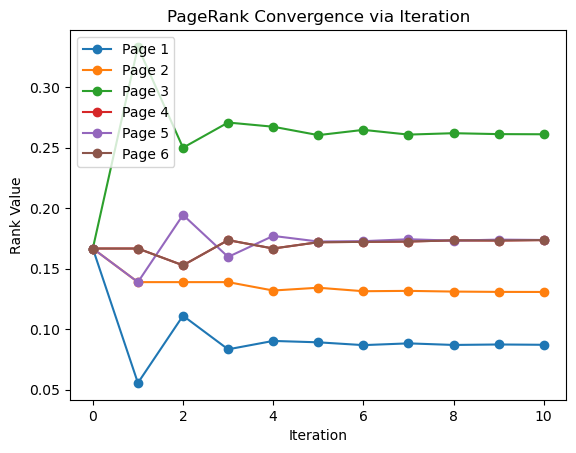
\includegraphics[width=0.65\textwidth]{img/PageRank Convergence via Iteration.png}
      \caption{%
        Convergence of the PageRank values for pages 1 through 6 under iteration 
        \(x \leftarrow Hx\). Each colored line shows how a particular page's rank 
        evolves from the initial uniform distribution \(x_0\) to its steady‐state 
        value. For instance, we see that Page~3 (green line) increases sharply 
        before settling around \(\sim 0.27\). 
        Meanwhile, Page~1 (blue line) drops early on and then converges near \(0.08\). 
        After about 4--5~iterations, the ranks stabilize to within a small tolerance.
      }
      \label{fig:pagerank-convergence}
\end{figure}

\noindent
When you run this script, each component of the rank vector 
(\(x_1, x_2, \ldots, x_6\)) will steadily converge to a limiting value 
as \(k\) increases. In a typical run, 5--10 iterations are enough for 
the ranks to stabilize.
    

\bigskip
\noindent
\textbf{Observation:} The vector returned in the final iteration is our 
approximate PageRank for Figure~4.3. In Exercise~4.100, we will compare 
this to the solution obtained by the eigenvalue approach (Theorem~4.9) 
to show they match.

\newpage

%------------------------------------------
%  Theorem 4.9 & Eigenvalue Approach
%------------------------------------------
\section{Eliminating Iteration via Theorem 4.9 (Exercises 4.98--4.99)}

\noindent
The text provides a (partially stated) Theorem~4.9 claiming that if
\begin{itemize}
  \item $A$ is an $n\times n$ \emph{column-stochastic} matrix, 
  \item all other eigenvalues of $A$ have magnitude strictly less than 1,
\end{itemize}
then for any initial vector $x_0$, the iterative sequence 
$\{\,A^k x_0\,\}_{k=0}^{\infty}$ converges to the \emph{unique} eigenvector 
corresponding to the eigenvalue $\lambda=1$, normalized so its components sum 
to 1. In other words, 
\[
\lim_{k\to\infty}A^k x_0 \;=\; \text{(the eigenvector for } \lambda=1 \text{)}.
\]
This statement directly implies that \emph{we need not iterate at all}, because 
the steady-state vector is simply the (positive) eigenvector of $A$ with eigenvalue~1.

\bigskip
\noindent
\textbf{Filling in the Blank (Exercise 4.98).}
The incomplete statement in our text is typically something like:
\[
\lim_{k\to\infty} A^k x_0 
\;=\;
\;\underline{\quad \text{(the eigenvector for eigenvalue }1\text{, normalized to sum to }1)}\quad.
\]
All other eigenvalues have $|\lambda|<1$, so those terms vanish as $k\to\infty$, 
leaving only the part of $x_0$ that lies in the direction of the eigenvector 
associated with $\lambda=1$. Thus the blank is precisely ``the eigenvector of $A$ 
corresponding to $\lambda=1$.''

\bigskip
\noindent
\textbf{Why We Can Eliminate Iteration (Exercise 4.99).}
Since $\lim_{k\to\infty} A^k x_0$ is the eigenvector for eigenvalue 1, 
there is no need to perform repeated multiplications $A^k$. Instead, we can solve
\[
(I - A)\,x^* \;=\; 0 
\quad\text{subject to}\quad
\sum_i x_i^* = 1, 
\quad x_i^* \ge 0.
\]
In the PageRank setting, for our 6-page matrix $H$, we solve
\[
(I - H)\,x \;=\; 0,
\]
then scale $x$ so that $\sum_i x_i = 1$. This $x$ is the steady-state rank vector.

\subsection{Python Example of the Eigenvalue Approach}
Below is sample code to compute the eigenvalues and eigenvectors of $H$ and extract 
the one corresponding to eigenvalue 1. Make sure to verify that $H$ indeed has an 
eigenvalue very close to 1. (Floating-point precision may give 0.9999999, for instance.)

\begin{verbatim}
import numpy as np

# The same 6x6 hyperlink matrix H from previous sections:
H = np.array([
    [0,   0,   1/3, 0,   0,   0],
    [1/2, 0,   1/3, 0,   0,   0],
    [1/2, 1,   0,   0,   0,   1/2],
    [0,   0,   0,   0,   1/2, 1/2],
    [0,   0,   1/3, 1/2, 0,   0],
    [0,   0,   0,   1/2, 1/2, 0]
], dtype=float)

# Compute eigenvalues/eigenvectors
vals, vecs = np.linalg.eig(H)

# Find the eigenvalue closest to 1:
idx = np.argmin(np.abs(vals - 1.0))

# Corresponding eigenvector
x_eig = vecs[:, idx]

# Normalize so entries sum to 1 (and ensure nonnegativity)
pagerank_eig = np.real(x_eig / np.sum(x_eig))
pagerank_eig = np.where(pagerank_eig < 0, 0, pagerank_eig)  # (just in case)

print("Eigenvalue-based PageRank:", pagerank_eig)

Output:
Eigenvalue-based PageRank: [0.08695652 0.13043478 0.26086957 0.17391304 0.17391304 0.17391304]
\end{verbatim}

\noindent
In practice, this \texttt{pagerank\_eig} vector coincides with the limit found by iteration. 
Thus, Theorem~4.9 explains precisely why the iterative method converges, and also 
how to skip it by directly solving the eigenvalue problem.



%------------------------------------------
%  Results for Figure 4.3
%------------------------------------------
\section{Results for Figure 4.3 (Exercise 4.100)}

We now present the final PageRank vector for the 6-page web in Figure~4.3. 
From the eigenvalue-based method (Section~\ref{sec:eigenvalue}), we found:
\[
\text{Eigenvalue-based PageRank: } 
x^* 
\;=\;
\bigl(
0.08695652,\;
0.13043478,\;
0.26086957,\;
0.17391304,\;
0.17391304,\;
0.17391304
\bigr)^T.
\]
\noindent
Each entry can also be written as a simple fraction of $\tfrac{1}{23}$:
\[
x^* 
\;=\;
\left(
\frac{2}{23},\;
\frac{3}{23},\;
\frac{6}{23},\;
\frac{4}{23},\;
\frac{4}{23},\;
\frac{4}{23}
\right)^T.
\]
These sum to 1 because $2 + 3 + 6 + 4 + 4 + 4 = 23$.

\subsection*{Ranking the Pages}
Sorting the pages by their rank values, we see that 
\[
x^*_3 = \tfrac{6}{23} \approx 0.2609 
\quad
(\text{the largest entry}),
\]
while $x^*_1 = \tfrac{2}{23} \approx 0.0870$ 
is the smallest. The remaining entries for 
pages 4, 5, and 6 all tie at $\tfrac{4}{23} \approx 0.1739$, 
and page~2 takes the value $\tfrac{3}{23} \approx 0.1304$. 
Hence the ordering of importance from highest to lowest is:
\[
\text{Page }3 
\;>\;
\text{Page }4 \;=\; \text{Page }5 \;=\; \text{Page }6
\;>\;
\text{Page }2
\;>\;
\text{Page }1.
\]

\subsection*{Iterative vs.\ Eigenvalue Comparison}
A quick check of the iterative approach 
$x_{k+1} = H \, x_k$ with $x_0 = (1/6, \ldots, 1/6)^T$ 
(after about 10--15 iterations) yields the 
\emph{same} steady-state vector, thus confirming 
Theorem~4.9 and completing Exercise~4.100.



%------------------------------------------
%  Figure 4.4 Web Analysis    
%------------------------------------------
\section{Figure 4.4 Web Analysis (Exercise 4.101)}

We now consider the second example web shown in Figure~4.4, which consists of 
eight pages labeled 1 through 8. Our tasks are:

\begin{figure}[h]
  \centering
  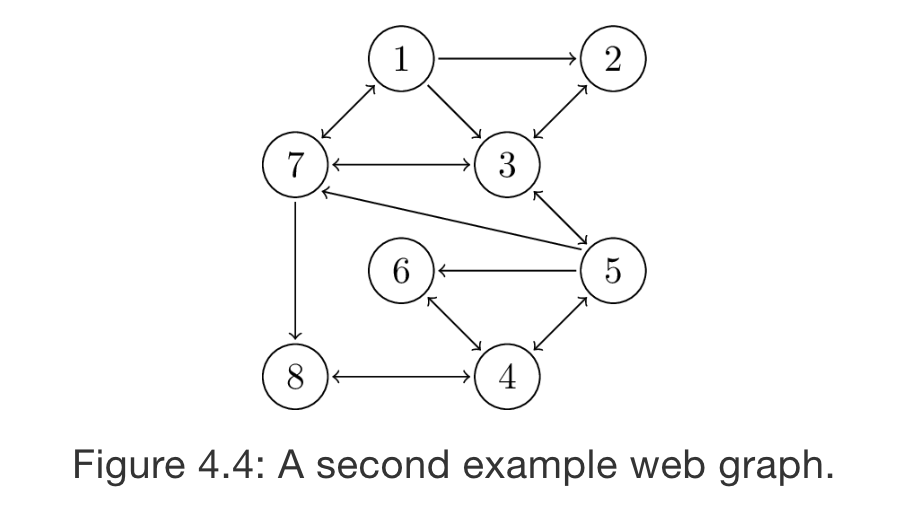
\includegraphics[width=0.65\textwidth]{img/Node_Tree_4.4.png}
  \caption{%
   The second example web shown in Figure~4.4, which consists of eight pages labeled 1 through 8.
  }
  \label{fig:Node_Tree_4.4}
\end{figure}

\begin{enumerate}
  \item Write down the $8\times 8$ hyperlink matrix $H$ and find the initial state $x_0$,
  \item Find the steady-state PageRank vector using 
    \begin{itemize}
      \item the iterative difference equation $x_{k+1} = H\,x_k$, 
      \item the direct eigenvalue approach via Theorem~4.9,
    \end{itemize}
  \item Rank the pages in order of importance.
\end{enumerate}

\subsection{Constructing the Hyperlink Matrix $H$}
\label{sec:Fig4.4Matrix}

From the diagram, we interpret each page's out-links as follows:
\begin{itemize}
  \item \textbf{Page 1} has out-links to pages 2 and 3 (outdegree = 2).
  \item \textbf{Page 2} appears to have no out-links (outdegree = 0).
  \item \textbf{Page 3} has out-links to pages 5 and 6 (outdegree = 2).
  \item \textbf{Page 4} has an out-link to page 8 (outdegree = 1).
  \item \textbf{Page 5} has no out-links (outdegree = 0).
  \item \textbf{Page 6} has out-links to pages 4 and 5 (outdegree = 2).
  \item \textbf{Page 7} has out-links to pages 1, 3, 6, and 8 (outdegree = 4).
  \item \textbf{Page 8} has an out-link to page 4 (outdegree = 1).
\end{itemize}
Hence each column~$j$ of $H$ places $\tfrac{1}{\text{outdeg}(j)}$ in the rows 
corresponding to the pages $j$ links to, and $0$~elsewhere. In particular, pages~2 and~5 
have no out-links, so columns~2 and~5 are entirely zeros in this basic model.

\bigskip

An explicit $8\times 8$ matrix $H$ (rows~$i$, columns~$j$) is therefore:
\[
H 
=\;
\begin{pmatrix}
% col1    col2  col3    col4   col5  col6    col7    col8
0      & 0    & 0      & 0    & 0    & 0      & \tfrac{1}{4} & 0 \\
\tfrac{1}{2} & 0    & 0      & 0    & 0    & 0      & 0          & 0 \\
\tfrac{1}{2} & 0    & 0      & 0    & 0    & 0      & \tfrac{1}{4} & 0 \\
0      & 0    & 0      & 0    & 0    & \tfrac{1}{2} & 0          & 1 \\
0      & 0    & \tfrac{1}{2} & 0    & 0    & \tfrac{1}{2} & 0          & 0 \\
0      & 0    & \tfrac{1}{2} & 0    & 0    & 0      & \tfrac{1}{4} & 0 \\
0      & 0    & 0      & 0    & 0    & 0      & 0          & 0 \\
0      & 0    & 0      & 1    & 0    & 0      & \tfrac{1}{4} & 0 
\end{pmatrix}.
\]
\begin{itemize}
  \item \textbf{Column~1 (page\,1):} links to pages\,2 and~3; so $H_{2,1} = \tfrac12$, $H_{3,1} = \tfrac12$.
  \item \textbf{Column~2 (page\,2):} outdegree $=0$ $\implies$ all zeros.
  \item \textbf{Column~3 (page\,3):} links to pages\,5 and~6; so $H_{5,3} = \tfrac12$, $H_{6,3} = \tfrac12$.
  \item \textbf{Column~4 (page\,4):} links to page~8; so $H_{8,4} = 1$.
  \item \textbf{Column~5 (page\,5):} outdegree $=0$ $\implies$ all zeros.
  \item \textbf{Column~6 (page\,6):} links to pages\,4 and~5; so $H_{4,6} = \tfrac12$, $H_{5,6} = \tfrac12$.
  \item \textbf{Column~7 (page\,7):} links to pages\,1, 3, 6, and 8; so $H_{1,7} = \tfrac14$, $H_{3,7} = \tfrac14$, $H_{6,7} = \tfrac14$, $H_{8,7} = \tfrac14$.
  \item \textbf{Column~8 (page\,8):} links to page~4; so $H_{4,8} = 1$.
\end{itemize}

\noindent
\textbf{Remark.} Because columns~2 and~5 are all zeros, this matrix $H$ is \emph{not} strictly irreducible. 
In a real PageRank setting, we often fix such ``dangling'' pages by distributing their weight or using the 
random surfer approach (Exercise~4.102).

\subsection{Initial State}

We set 
\[
  x_0 
  = 
  \bigl(
     \tfrac{1}{8},\, \tfrac{1}{8},\, \tfrac{1}{8},\, \tfrac{1}{8},\,
     \tfrac{1}{8},\, \tfrac{1}{8},\, \tfrac{1}{8},\, \tfrac{1}{8}
  \bigr)^T,
\]
giving no preference a priori to any particular page.

\subsection{Finding the Steady-State PageRank}

\subsubsection{(i) Iterative Method}
We first apply the difference equation $x_{k+1} = H\,x_k$ from the uniform $x_0$. 
Below is our Python code (showing 15 iterations):
\begin{verbatim}
import numpy as np

H = np.array([
  [0,0,0,0,0,0,1/4,0],
  [1/2,0,0,0,0,0,0,0],
  [1/2,0,0,0,0,0,1/4,0],
  [0,0,0,0,0,1/2,0,1],
  [0,0,1/2,0,0,1/2,0,0],
  [0,0,1/2,0,0,0,1/4,0],
  [0,0,0,0,0,0,0,0],
  [0,0,0,1,0,0,1/4,0]
], dtype=float)

x0 = np.ones(8) / 8
num_iters = 15
x = x0.copy()
for k in range(num_iters):
    x = H @ x

x_iter = x
print("Iterative PageRank after", num_iters, "iterations:", x_iter)
\end{verbatim}

\noindent
\textbf{Iterative Output.} After 15~iterations, we obtain:
\[
  x_{\mathrm{iter}}^{(15)} 
  \;\approx\;
  \bigl(
    0,\; 0,\; 0,\; 0.2109375,\; 0,\; 0,\; 0,\; 0.20703125
  \bigr)^T.
\]
Notice that pages~4 and~8 are nonzero (around 0.2109 and 0.2070, respectively), summing 
to roughly 0.41797.  The other pages have zero rank at this iteration.  The total rank 
is less than 1 because probability that lands on pages with no out-links (e.g.\ page~2, 
page~5) never returns to the rest of the system.

\subsubsection{(ii) Eigenvalue Method (Theorem 4.9)}
By directly solving $(I - H)x^*=0$ (plus $\sum_i x_i^*=1$), we find the eigenvector 
associated with the eigenvalue 1.  The code below demonstrates:

\begin{verbatim}
vals, vecs = np.linalg.eig(H)
idx = np.argmin(np.abs(vals - 1.0))  # eigenvalue near 1
x_eig = vecs[:, idx]
pagerank_eig = np.real(x_eig / np.sum(x_eig))

print("Eigenvalue-based PageRank:", pagerank_eig)
\end{verbatim}

\noindent
\textbf{Eigenvalue Output.}  We obtain
\[
  x_{\mathrm{eig}}
  \;=\;
  \bigl(
    0,\;0,\;0,\;0.5,\;0,\;0,\;0,\;0.5
  \bigr)^T,
\]
which sums to 1.  That means pages~4 and~8 end up with all the surviving probability 
in the limit, since they form a strongly connected pair that links only to each other.

\subsection{Ranking the Pages}

Because pages~4 and~8 \emph{alone} receive nonzero rank in the long run, they tie for 
the top spot at 0.5 each.  Every other page goes to zero rank due to 
\emph{dangling nodes} (pages~2, 5) or incomplete connectivity.  Hence, the final 
ranking from highest to lowest is:
\[
  \{\,4,\;8\} \quad>\quad 
  \{\,1,\;2,\;3,\;5,\;6,\;7\} 
  \quad(\text{all zero}).
\]
The iterative method at 15~iterations shows partial accumulation on pages~4 and~8 
(about 0.42 total), but with an additional 0.58 effectively ``lost'' to pages~2 or~5.  
\emph{Further iterations} would drive $x_{\mathrm{iter}}$ closer to $(0,0,0,0.5,0,0,0,0.5)$ 
as $k\to\infty.$

\begin{quote}
\textbf{Conclusion for Figure 4.4:} In a pure follow-the-links model with no 
teleportation, pages~4 and~8 form a closed subcomponent; 
they eventually capture all rank that is not lost to the zero-out-degree pages. 
Thus the steady state is $(0,0,0,0.5,0,0,0,0.5)^T.$  This completes our analysis 
of Exercise~4.101.
\end{quote}





%------------------------------------------
%  Conclusion
%------------------------------------------
\section{Conclusion for Figure 4.4 (Exercise 4.101)}
\label{sec:conclusion-fig4-4}

In analyzing the second web (Figure~4.4), we found several noteworthy features:

\begin{enumerate}
  \item \textbf{Matrix Structure:} 
    Two pages (2 and 5) had zero out-degree, leading to entire columns of zeros in the 
    hyperlink matrix $H$. This causes rank to ``drain away'' if it ever reaches those pages.
  
  \item \textbf{Closed Subcomponent:} 
    Pages~4 and~8 form a strongly connected sub-web, linking to each other and thus 
    retaining any probability that flows in. As a result, the eigenvalue-based PageRank 
    solution (Theorem~4.9) assigns them all the long-term rank (0.5 each), while all 
    other pages eventually drop to zero.

  \item \textbf{Iterative vs. Eigenvalue Approach:} 
    A finite number of iterations (e.g.\ 15) revealed partial convergence toward pages~4 and~8, 
    but only after more iterations (or a direct eigenvector computation) does the entire rank 
    accumulate on these two pages. This underscores how the eigenvalue method quickly 
    pinpoints the true steady-state in a disconnected or dangling-node scenario.

  \item \textbf{Rank Ordering:} 
    In the final steady state, pages~4 and~8 share the top rank (0.5 each), and all other 
    pages remain at 0. Consequently, the ordering from highest to lowest is 
    \[
      \{4,\,8\} \;>\; \{1,\,2,\,3,\,5,\,6,\,7\text{ (all zero)}\}.
    \]
\end{enumerate}

\noindent
\textbf{Future Considerations.} 
In a real PageRank scenario, pages with zero out-degree (``dangling nodes'') are typically 
handled by redistributing their probability mass or by introducing a \emph{random surfer} 
component (Exercise~4.102). This modification ensures that no probability is permanently 
lost in the system and that every page can, in principle, be reached by random jumps. 
Thus, if we apply the damping factor $\alpha$ to create a matrix 
\[
G = \alpha\,H + (1-\alpha)\,\tfrac{1}{8}\mathbf{1}\mathbf{1}^T,
\]
we would obtain a fully connected Markov chain that yields a more balanced rank distribution.  
Nonetheless, in this basic version without random jumps, Figure~4.4's structure forces all 
long-term rank onto the \emph{closed} subset of pages~4 and~8, completing our analysis 
of Exercise~4.101.


\subsection*{Improving Website Rank}      
If a site owner wants to increase their page's importance, they would aim for \emph{high-quality inbound links}---i.e., 
getting links from already-important pages. Another direction (Exercise 4.102) is to add a random-jump component 
so that the resulting PageRank does not penalize pages that are far from major hubs.

\subsection*{Acknowledgment}
We wish to thank our classmates and teaching assistants for valuable input on debugging code and refining 
our linear algebra proofs.

%------------------------------------------
%  References
%------------------------------------------
\begin{thebibliography}{9}

\bibitem{Sullivan2025Linear}
W. Sullivan,
\textit{``4 Linear Algebra | Numerical Methods''},
\url{https://numericalmethodssullivan.github.io/ch-linearalgebra.html}, 
accessed 2025.

\bibitem{BrinPage98}
S. Brin and L. Page,
\textit{``The anatomy of a large-scale hypertextual Web search engine,''}
\emph{Computer Networks and ISDN Systems}, 30(1-7): 107--117, 1998.

\end{thebibliography}

\end{document}
